\documentclass[12pt,a4paper]{article}
\usepackage{fontspec, xunicode, xltxtra}
\setmainfont{SimSun}
\usepackage{indentfirst} 
\XeTeXlinebreaklocale "zh"
\usepackage[left=2.5cm,right=2.5cm,top=2.5cm,bottom=2.5cm]{geometry}
\usepackage{changepage}
\usepackage{float}
\usepackage{setspace}
\usepackage{amsmath}
\usepackage{amsfonts}
\usepackage{amssymb}
\usepackage{circuitikz}
\usepackage{graphicx}

\title{实验三\quad 负反馈放大电路}
\author{自54 田毅\\ 2015011451}

\graphicspath{{Figure/}}
\begin{document}
\begin{spacing}{1.3}

\maketitle
\tableofcontents
\newpage
\section{实验目的}
\begin{enumerate}
\item 熟悉负反馈放大电路的组态;
\item 深入理解负反馈对放大电路性能的影响;
\item 进一步熟练掌握基于 Multisim 的仿真以及硬件电路的调试和性能测试方法。
\end{enumerate}
\section{预习报告}
\subsection{电压并联负反馈放大电路}
\subsubsection{理论估算}
\begin{figure}[H]
\centering
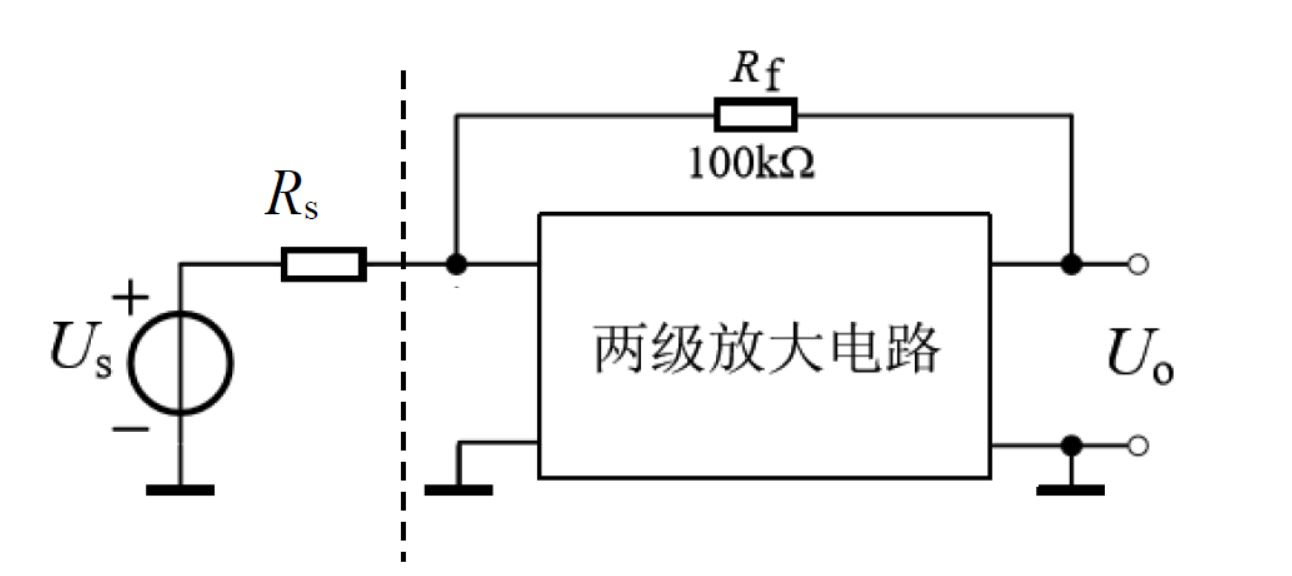
\includegraphics[width=10cm]{1.jpg}
\end{figure}
假设引入了深度负反馈,则
\[
\dot{A_{usf}} \approx \frac{1}{\dot{F_{iu}}} \cdot \frac{1}{R} = - \frac{R_f}{R} = -10
\]
因此选取$R_f = 10k\Omega$。根据“两级放大电路”实验中硬件实验中测试结果及实验中电路元件取值,即$R_{g1} = R_{g2} = 220k\Omega, R_s = 4.51k\Omega$ ,有,
% $\begin{cases}
% \dot{A_{u1}} = \frac{g_m R_{o1}//R_{i2}}{1+g_m R_{o1}//R_{i2}} \approx \\
% \end{cases}$
\[
\dot{A_{ui}} = \frac{\dot{U_o}}{\dot{I_i}} = \frac{\dot{U_o} R_{i}}{\dot{U_i}} = \dot{A_u} R_{i},\dot{F_{iu}} = \frac{\dot{I_f}}{\dot{U_o}} = - \frac{1}{R_f}
\]
其中$\dot{A_{ui}}$测量结果为-159.6,$R_{i}$为考虑反馈网络负载效应后的输入电阻,$R_{i} = R // (R_{g3} + R_{g1} // R_{g2}) = 91.07k\Omega$,因此
\[
1 + \dot{A_{ui}} \dot{F_{iu}} \approx 1 + 159.6 \times \frac{91.07}{100} = 146.3 >> 1
\]
可见对于深度负反馈的假设合理。引入深度负反馈后,
\begin{center}
$\begin{cases}
R_{if} = \frac{R_i}{1 + AF}  = \frac{91.07 \times 10^3}{146.3} \approx 622.5\Omega\\
R_{of} = \frac{R_o}{1 + AF} = \frac{3.3 \times 10^3}{146.3} \approx 22.6\Omega
\end{cases}$
\end{center}
但是,我们注意到,$22.6\Omega$与后续的仿真及实验值相差很大,分析原因,在于$内阻R_s$的分流,应修正为
\[
R_{of} = \frac{R_o}{1 + AF \times \frac{R_S}{R_S+R_i}} = \frac{3.3 \times 10^3}{146.3\times \frac{10}{10+91.07}} \approx 228.0\Omega
\]

\subsubsection{仿真实验}
\begin{figure}[H]
\centering
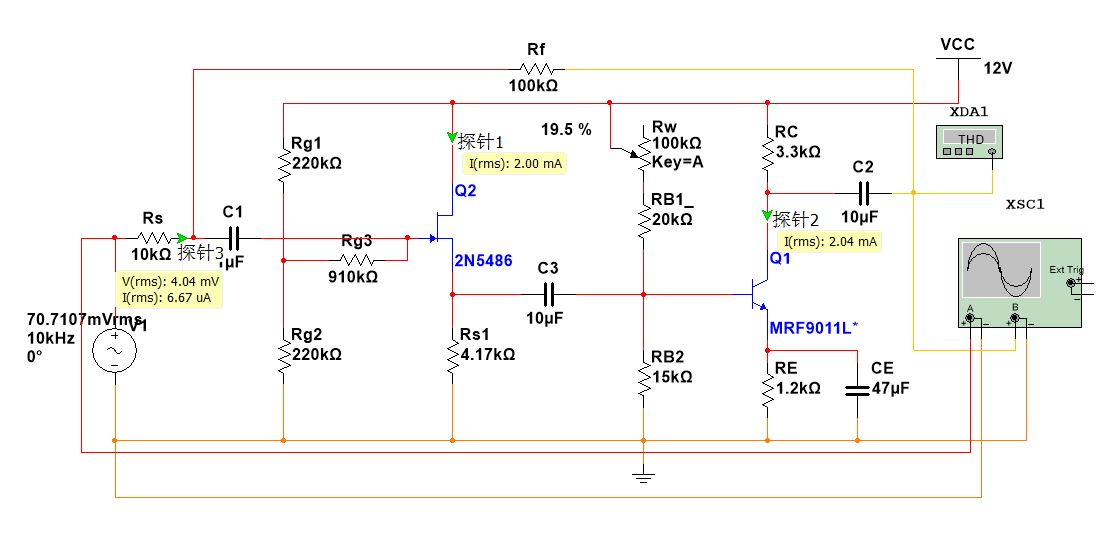
\includegraphics[width=\textwidth]{2.jpg}
\end{figure}
由图中探针可知,负反馈并未对静态工作点造成影响,首先用示波器测得输入输出波形如下:
\begin{figure}[H]
\centering
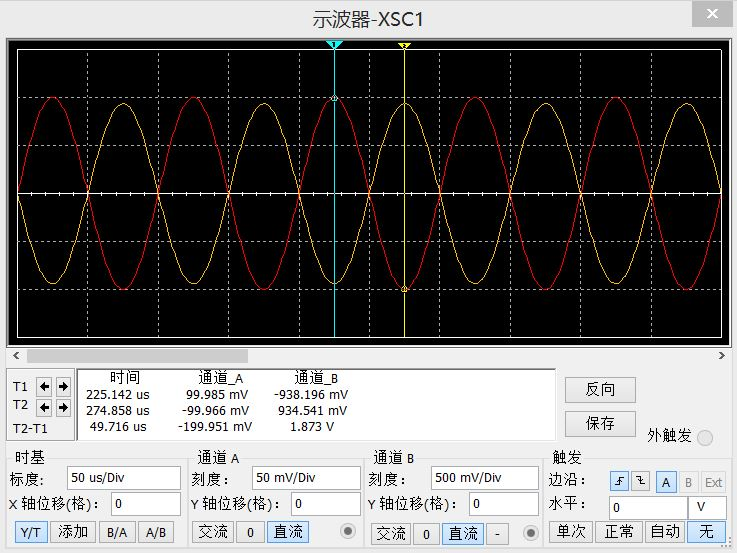
\includegraphics[width=\textwidth]{3.jpg}
\end{figure}
测得
\[
\dot{A_{usf}} = - \frac{\dot{U_o}}{\dot{U_s}} = - \frac{1.873}{199.951 \times 10^{-3}} \approx -9.37
\]
与理论的-10较为接近。同时可以看到,波形未出现失真。失真分析仪显示如下:
\begin{figure}[H]
\centering
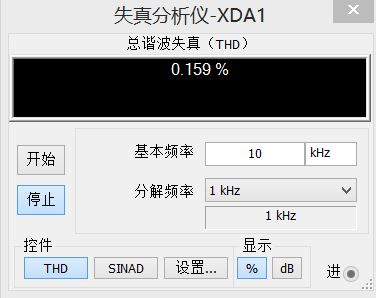
\includegraphics[width=8cm]{5.jpg}
\end{figure}
进一步地,通过探针测出输入电阻
\[
R_i = \frac{U'_i}{I_i} = \frac{4.04 \times 10^{-3}}{4.67 \times 10^{-4}} \approx 605.7\Omega
\]
输出端开路时,输出电压有效值$662mV$;在输出端接$R_L = 500\Omega$的负载电阻后,输出电压有效值$448mV$,计算出输出电阻
\[
R_o = (\frac{U_o}{U'_o}-1)R_L = (\frac{662}{448}-1)\times 500 = 238.8\Omega
\]
使用交流分析功能,测得电路的幅频特性如下:
\begin{figure}[H]
\centering
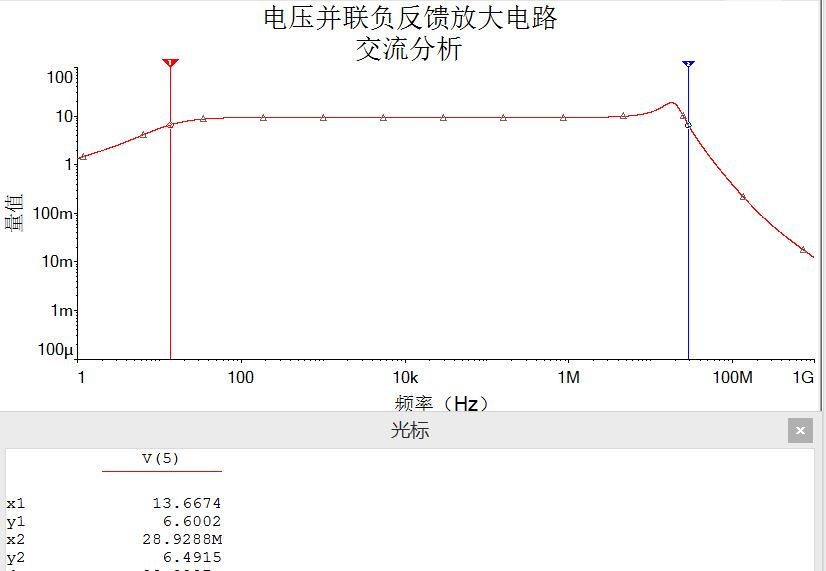
\includegraphics[width=\textwidth]{4.jpg}
\end{figure}
中频幅值为$9.37,降为0.707$倍的截止频率分别为
\[f_L \approx 13.67Hz,f_H \approx 28.93MHz\]
\subsection{电流并联负反馈放大电路}
\subsubsection{理论估算}
\begin{figure}[H]
\centering
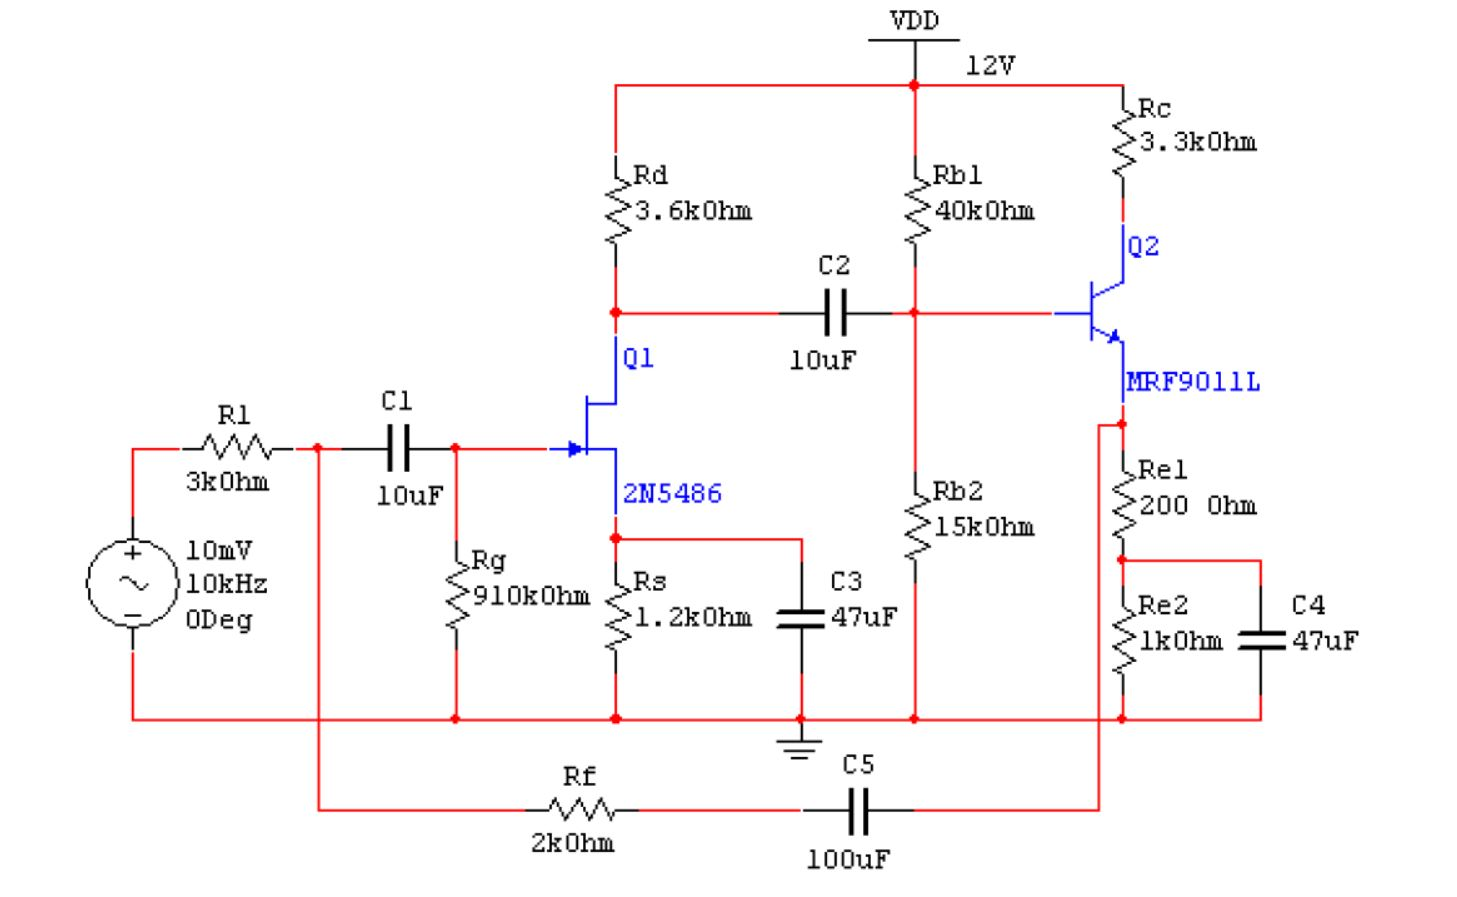
\includegraphics[width=12cm]{6.jpg}
\end{figure}
\paragraph{}静态动作点\\\\
对于第一级放大电路,忽略栅极电流,有
\begin{center}
$\begin{cases}
U_{GQ} = 0\\
U_{SQ} = I_{DQ}R_s\\
I_{DQ} = I_{DSS}(1-\frac{U_{GSQ}}{U_{GS(off)}})^2
\end{cases}$
\end{center}
由以上方程组,根据“两级放大电路”实验仿真测出的$I_{DSS} \approx 14.473mA,U_{GS(off) \approx -3.77V}$,解出
\[
I_{DQ} \approx 1.98mA,U_{GSQ} \approx -2.376V
\]
对于第二级放大电路,有
\begin{center}
$\begin{cases}
U_{BQ} \approx \frac{R_{b2}}{R_{b1}+R_{b2}} V_{DD}\\
U_{BQ} = U_{BEQ} + I_{EQ}(R_{e1}+R_{e2})\\
I_{CQ} = \frac{\beta}{1+\beta} I_{EQ}
\end{cases}$
\end{center}
解上述方程组,$U_{BEQ}\approx 0.7V$,代入“单管放大电路”实验仿真测量结果$\beta \approx 214$,解得
\[
U_{BQ} = 3.27V,I_{EQ}\approx 2.14mA,I_{CQ}\approx 2.13mA
\]
由此计算出
\begin{center}
$\begin{cases}
U_{CQ} = V_{DD}-I_{CQ}\cdot R_c \approx 4.971V\\
U_{EQ} = I_{EQ}\cdot (R_{e1}+R_{e2}) \approx 2.568V\\
U_{CEQ} = U_{CQ} - U_{EQ} \approx 2.403V
\end{cases}$
\end{center}
\paragraph{}动态参数\\\\
场效应管的跨导
\[
g_m = \frac{2}{|U_{GS(off)}|}\sqrt{I_{DQ}I_{DSS}} \approx 2.84mS
\]
晶体管$r_{bb'}取100\Omega$,则有
\[
r_{be} \approx r_{bb'} + \frac{\beta U_T}{I_{CQ}} \approx  2.71k\Omega
\]
考虑负载效应,由此计算出两级的开环放大倍数分别为:
\[
\dot{A_{u1}} = -g_m\{R_d//R_{b1}//R_{b2}//[r_{be}+(1+\beta)(R_{e1}//R_f)]\} \approx -7.22
\]
\[
\dot{A_{u2}} = -\frac{\beta R_c}{[r_{be}+(1+\beta)(R_{e1}//R_f)]} \approx -16.89
\]
则基本放大电路的开环放大倍数
% 注:考虑负载效应时,电流负反馈I_o视作0
\[
\dot{A_{ii}} = \frac{\dot{I_o}}{\dot{I_i}} = -\frac{\dot{U_o}}{\dot{U'_i}} \cdot \frac{R_g}{R_c} = -\dot{A_{u1}} \cdot \dot{A_{u2}} \cdot \frac{R_g}{R_c}
\]
反馈系数
\[
\dot{F_{ii}} = \frac{\dot{I_f}}{\dot{I_o}} = -\frac{R_{e1}}{R_{e1}+R_f} = -\frac{1}{11}
\]
因此$1 + \dot{A_{ii}}\dot{F_{ii}}\approx 121.9 >> 1$,故可认为引入深度负反馈,闭环电压放大倍数为
\[
\dot{A_{usf}} \approx -\frac{1}{\dot{F_{ii}}}\cdot \frac{R_c}{R_1} = 12.1
\]
输入电阻
\[
R_i = \frac{R_g}{1 + \dot{A_{ii}} \frac{R_g}{R_c} \dot{F_{ii}}} \approx 297.7\Omega
\]
输出电阻
\[
R_o = R_c = 3.3k\Omega
\]
\subsubsection{仿真实验}
\begin{figure}[H]
\centering
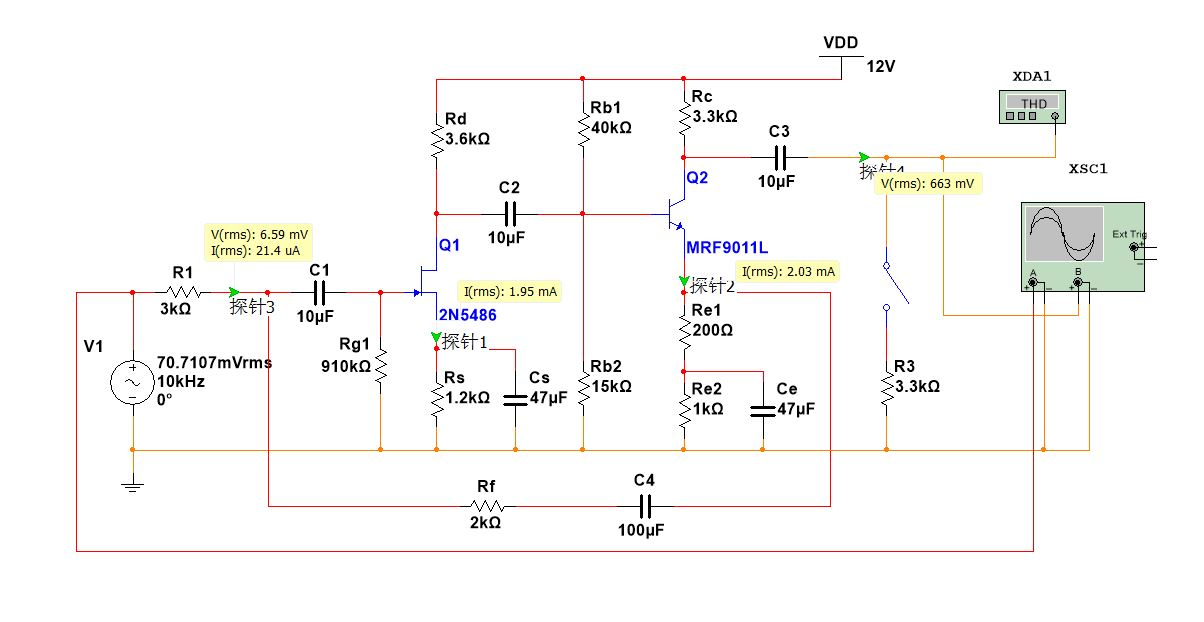
\includegraphics[width=\textwidth]{7.jpg}
\end{figure}
仿真电路如上所示。输入峰-峰值$200mV、10kHz$的交流电压,得到波形如下:
\begin{figure}[H]
\centering
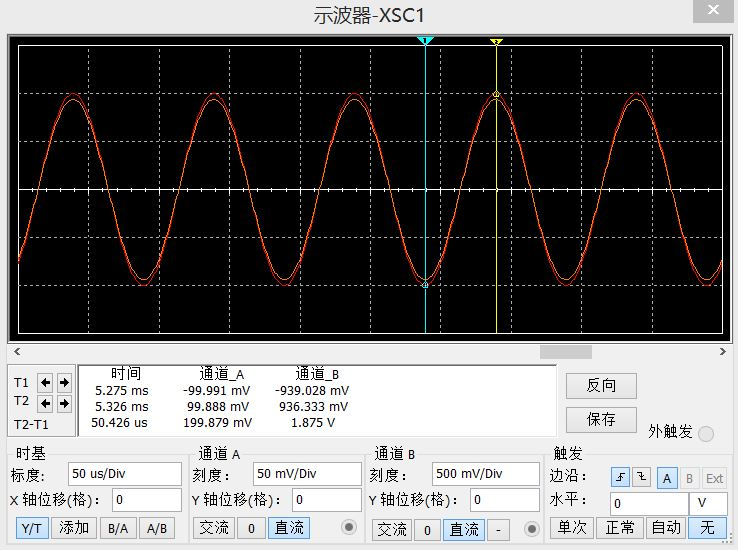
\includegraphics[width=\textwidth]{8.jpg}
\end{figure}
由示波器波形看出输入、输出电压同相,测得电压放大倍数为
\[
\dot{A_u} = \frac{\dot{U_o}}{\dot{U_i}} = \frac{1.875}{199.879\times 10^{-3}} \approx 9.38
\]
从波形也可看出在此情况下没有出现失真,这可从失真分析仪结果得到佐证:
\begin{figure}[H]
\centering
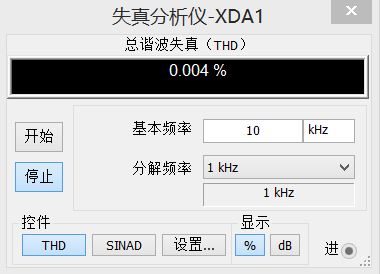
\includegraphics[width=8cm]{9.jpg}
\end{figure}
用与必做实验同样的方法,测得输入电阻
\[
R_i = \frac{U'_i}{I_i} = \frac{6.59}{21.4 \times 10^{-3}} \approx 307.95\Omega
\]
输出端开路$U_o = 663mV$,输出端接$R_L=3.3k\Omega$负载电阻时输出电压$U'_o = 333mV$,因此输出电阻
\[
R_o = (\frac{U_o}{U'_o}-1)\cdot R_L \approx 3.27k\Omega
\]
\section{注意事项}
\begin{enumerate}
\item 实验中要将学习机、信号源、示波器等电子仪器和实验电路共地,以免引起干扰。
\item 测量放大电路的各项动态特性时,要始终用示波器监视输入、输出波形。只有在输入输出信号不失真的情况下进行测量才有意义。
\item 输入电阻 $R_{if} 指图 1 中虚线右侧放大电路的输入电阻,不含 R_s$ 。
\item 引入电压负反馈后,输出电阻 $R_{of}$ 的数值较小。在实际测量时,为了防止因负载电流过大而烧坏管子,接在输出端的负载电阻建议不小于500 $\Omega$。
\end{enumerate}
\section{硬件实验}
\subsection{两级放大电路的恢复调试}
开环放大电路采用实验二中的两级放大电路。为了比较开环和闭环电路的动态参数,考虑图 1 中引入电压负反馈后反馈网络的负载效应,在该两级放大电路的输入端和输出端分别并联了与反馈电阻 $R_f$ 阻值相同的电阻 $R 和 R_L$ 。
首先对该两级放大电路的静态和动态参数进行恢复调试,确保其可以正常工作并满足前述参数要求。
\subsection{引入电压并联负反馈}
在上述两级放大电路中, 去除输入端和输出端 的电阻 $R 和 和 R_L$ ,然后正确引入电压并联负反馈。请合理选取电阻 $R_s$ 的阻值,使得闭环电压放大倍数的数值约为 10。

\subsection{负反馈放大电路的闭环测试}
\subsubsection{动态参数}
输入正弦信号 $U_s$ ,幅度为 $200mV,频率为 10kHz$,测量并记录闭环电压放大倍数$\dot{A_{usf}}=\frac{\dot{U_o}}{\dot{U_s}}$、输入电阻 $R_{if}$ 和输出电阻 $R_{of}$。\\
\paragraph{闭环放大倍数} 实验测得输入、输出波形如下。
\begin{figure}[H]
\centering
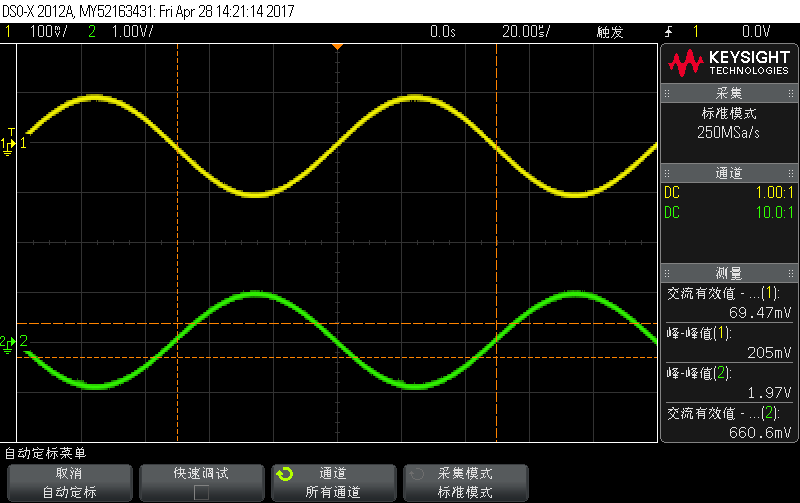
\includegraphics[width=\textwidth]{scope_0.png}
\end{figure}
由此计算出$\dot{A_{usf}}=\frac{660.4}{69.48}\approx 9.50$实验中,交流有效值等电学量有$0.1mV$级别的微小抖动,计算中使用这一抖动的均值,因此计算中数值与截图中数值可能有$0.1mV$级的差别。后面不再特别为此做出说明。
\paragraph{输入电阻} 输入电阻采用在$R_s$后串接$R_1=680\Omega$的方法进行测量。\\
串接后,$R_1$与输入总分压有效值$U_{i}^{'}=23.7mV$,输入部分两端分压$U_{i}^{''}=11.9mV$,波形图分别如下。
\begin{figure}[H]
\centering
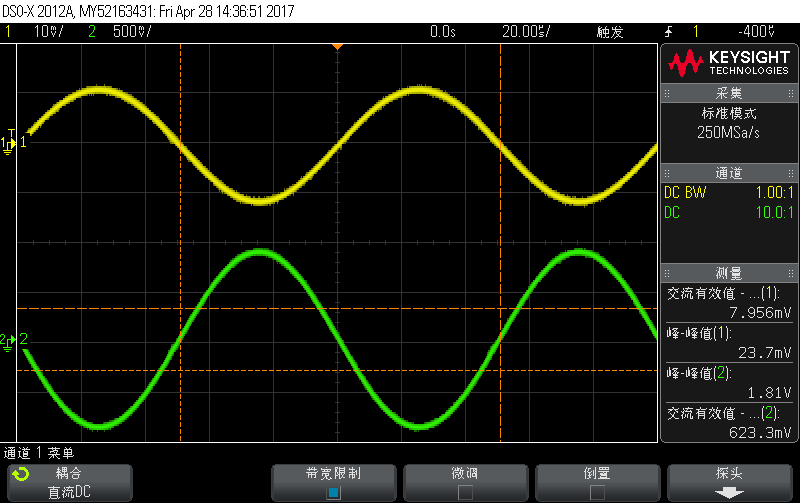
\includegraphics[width=\textwidth]{scope_2.png}
\end{figure}
\begin{figure}[H]
\centering
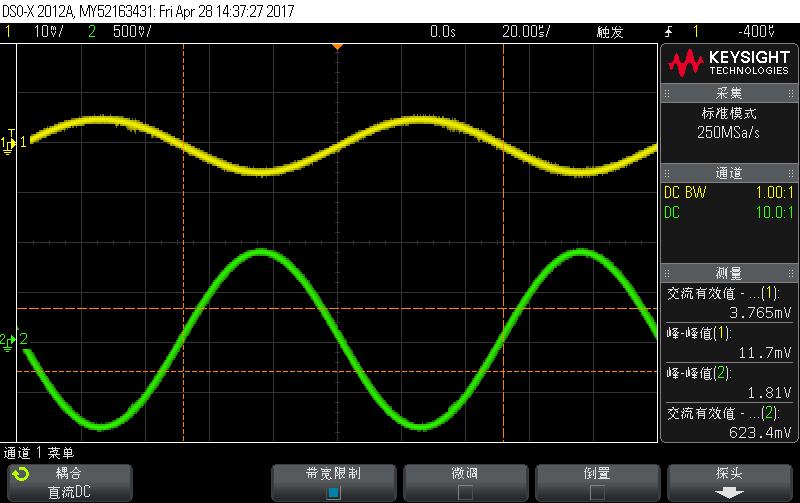
\includegraphics[width=\textwidth]{scope_3.png}
\end{figure}
据此计算出$R_{if}=\frac{11.9}{23.7-11.9}\times 680 \approx 685.76\Omega$。\\
\paragraph{输出电阻} 输出端开路时,$U_o=663.0mV$;在输出端接入$R_L=390\Omega$电阻,测得$U_{o}^{'}=419.0mV$,波形如下。
\begin{figure}[H]
\centering
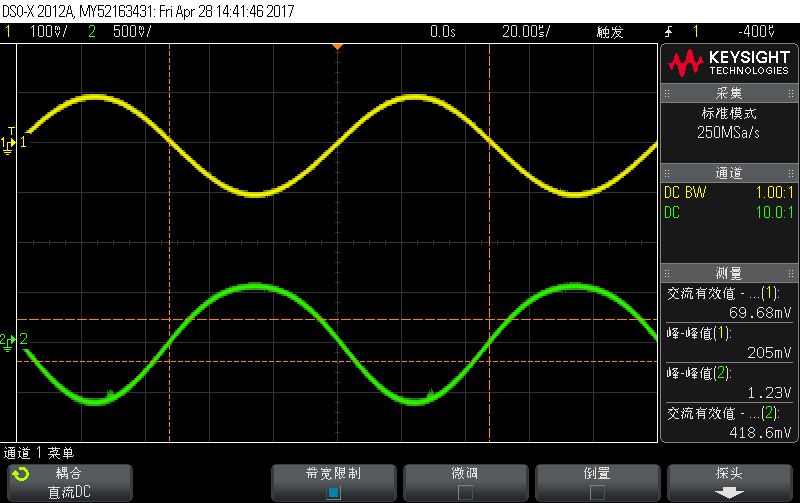
\includegraphics[width=\textwidth]{scope_4.png}
\end{figure}
据此计算出$R_{of} = (\frac{663.0}{419.0}-1)\times 390 = 227.1\Omega$。\\\\
最后将理论、仿真、实验值整理为如下表格。可以看到,实验与理论、仿真符合得相当好。
\begin{table}[H]
\centering
\begin{tabular}{|c|c|c|c|}
% hline draws a horizontal line
\hline 
&$\dot{A_{usf}}$ &$R_{if}(\Omega)$ &$ R_{of}(\Omega)$ \\ \hline 
理论值 &$-10 $& $ 622.5$ &$228.0 $\\ \hline
仿真值&$ -9.37$& $605.7 $ &$238.8 $\\ \hline 
实验值&$ -9.50$& $685.76 $ &$227.1 $\\ \hline
\end{tabular} 
\end{table} 
\subsubsection{截止频率}
对负反馈放大电路的上限截止频率 $f_H 和下限截止频率 f_L$ 进行测量,并和两级放大电路的测试结果进行比较。\\
在中频时,测得$U_o=663.0mV$,因此分别降低、升高频率,测得在$\frac{U_o}{\sqrt{2}}\approx 468.8mV$时,$f_L=13.5Hz,f_H=1.311MHz$。波形图分别如下所示。
\begin{figure}[H]
\centering
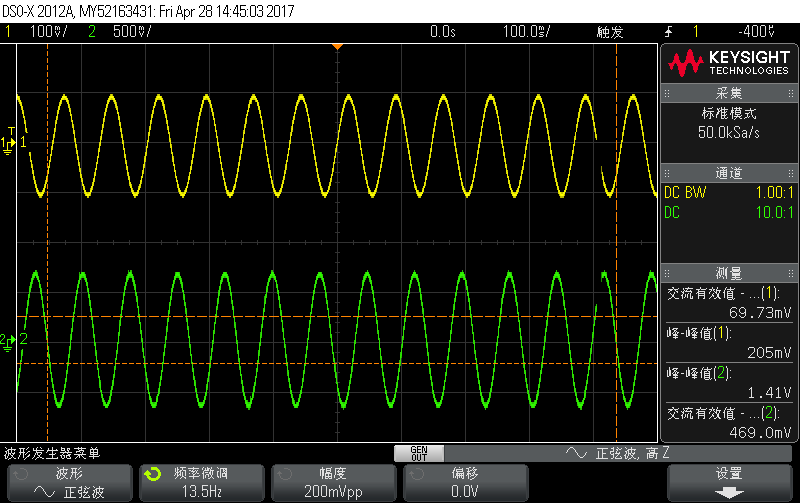
\includegraphics[width=\textwidth]{scope_5.png}
\end{figure}
\begin{figure}[H]
\centering
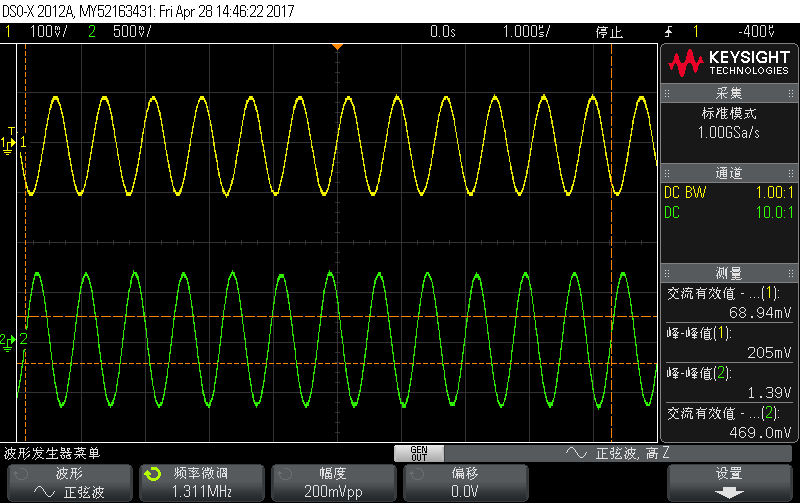
\includegraphics[width=\textwidth]{scope_6.png}
\end{figure}
\subsection{电流并联负反馈放大电路的测试研究}
输入正弦信号 $U_s ,幅度为 200mV,频率为 10kHz$,测量并记录闭环电压放大倍数$\dot{A_{usf}}=\frac{\dot{U_o}}{\dot{U_s}}$、输入电阻 $R_{if} 和输出电阻 R_{of}$。
\paragraph{电压放大倍数} 波形如下。据此计算出$\dot{A_{usf}} = \frac{609.1}{68.80} \approx 8.85$。
\begin{figure}[H]
\centering
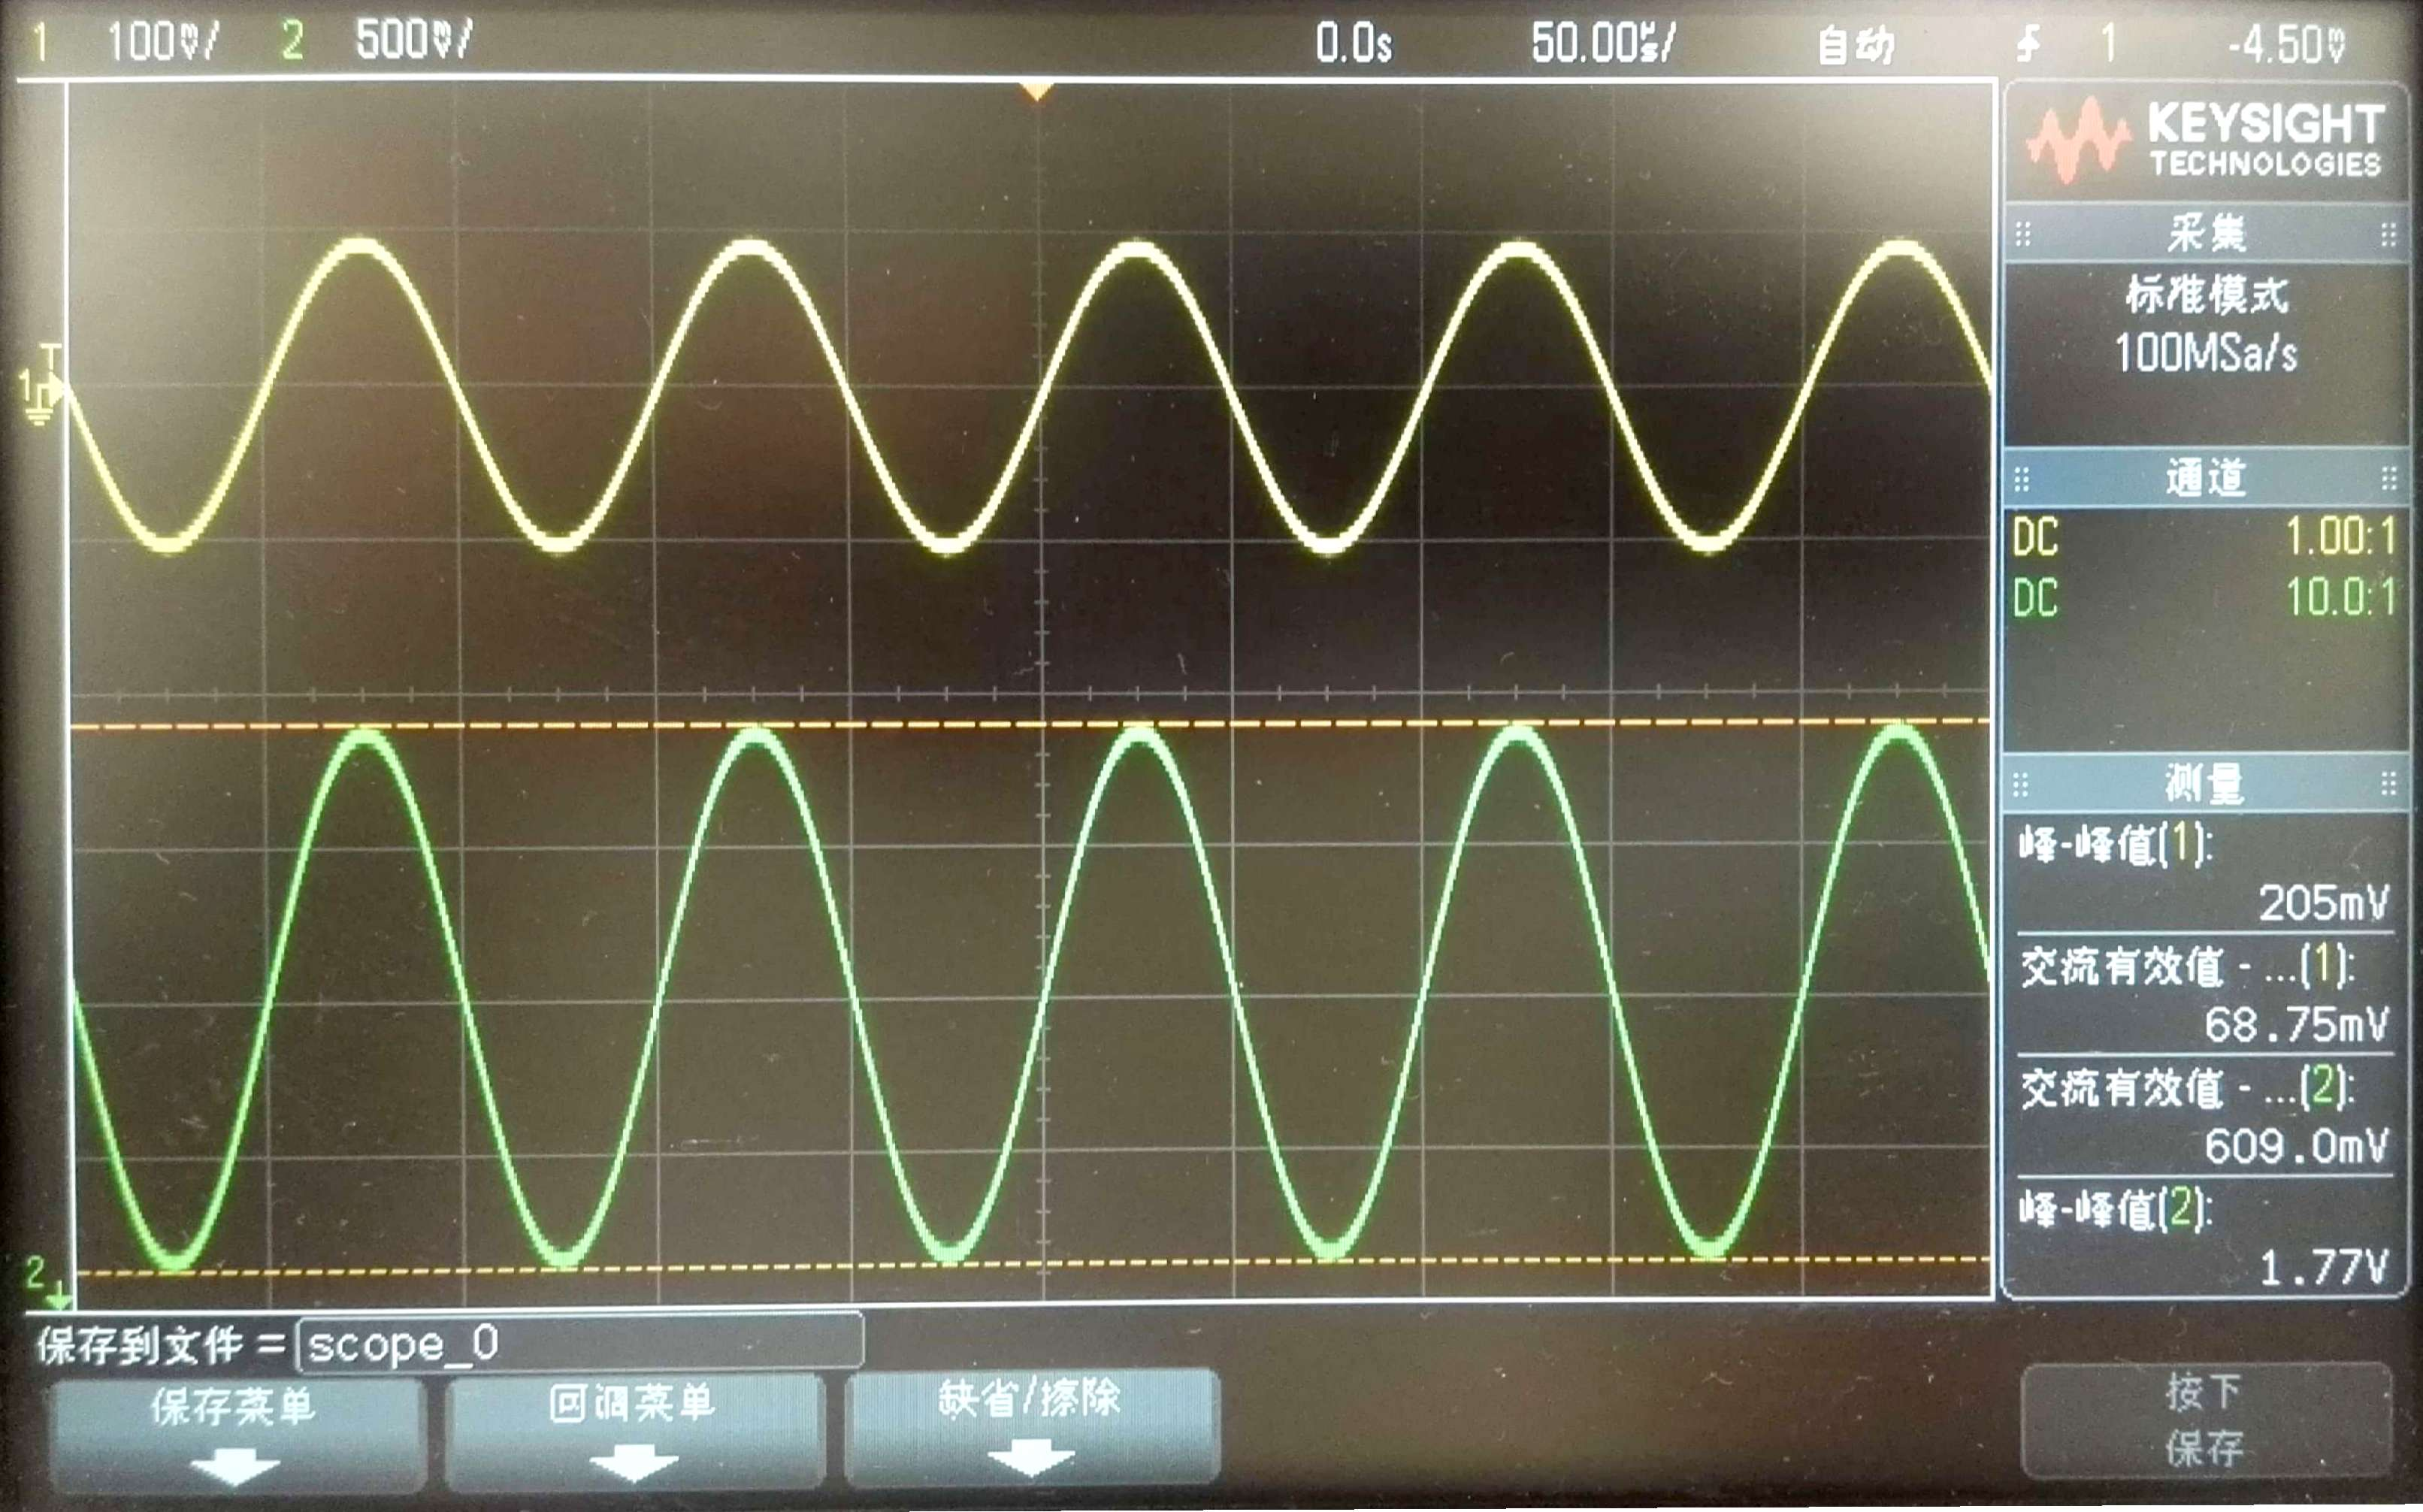
\includegraphics[width=\textwidth]{pic1.jpg}
\end{figure}
\paragraph{输入电阻} 方法与必做实验相同。$R_1=680\Omega$和输入部分总分压$U_{i}^{'}=17.72mV$,输入部分分压$U_{i}^{''}=6.27mV$,据此计算出$R_{if}=\frac{6.27}{17.72-6.27}\times 680 = 372.4\Omega$。波形图分别如下所示。
\begin{figure}[H]
\centering
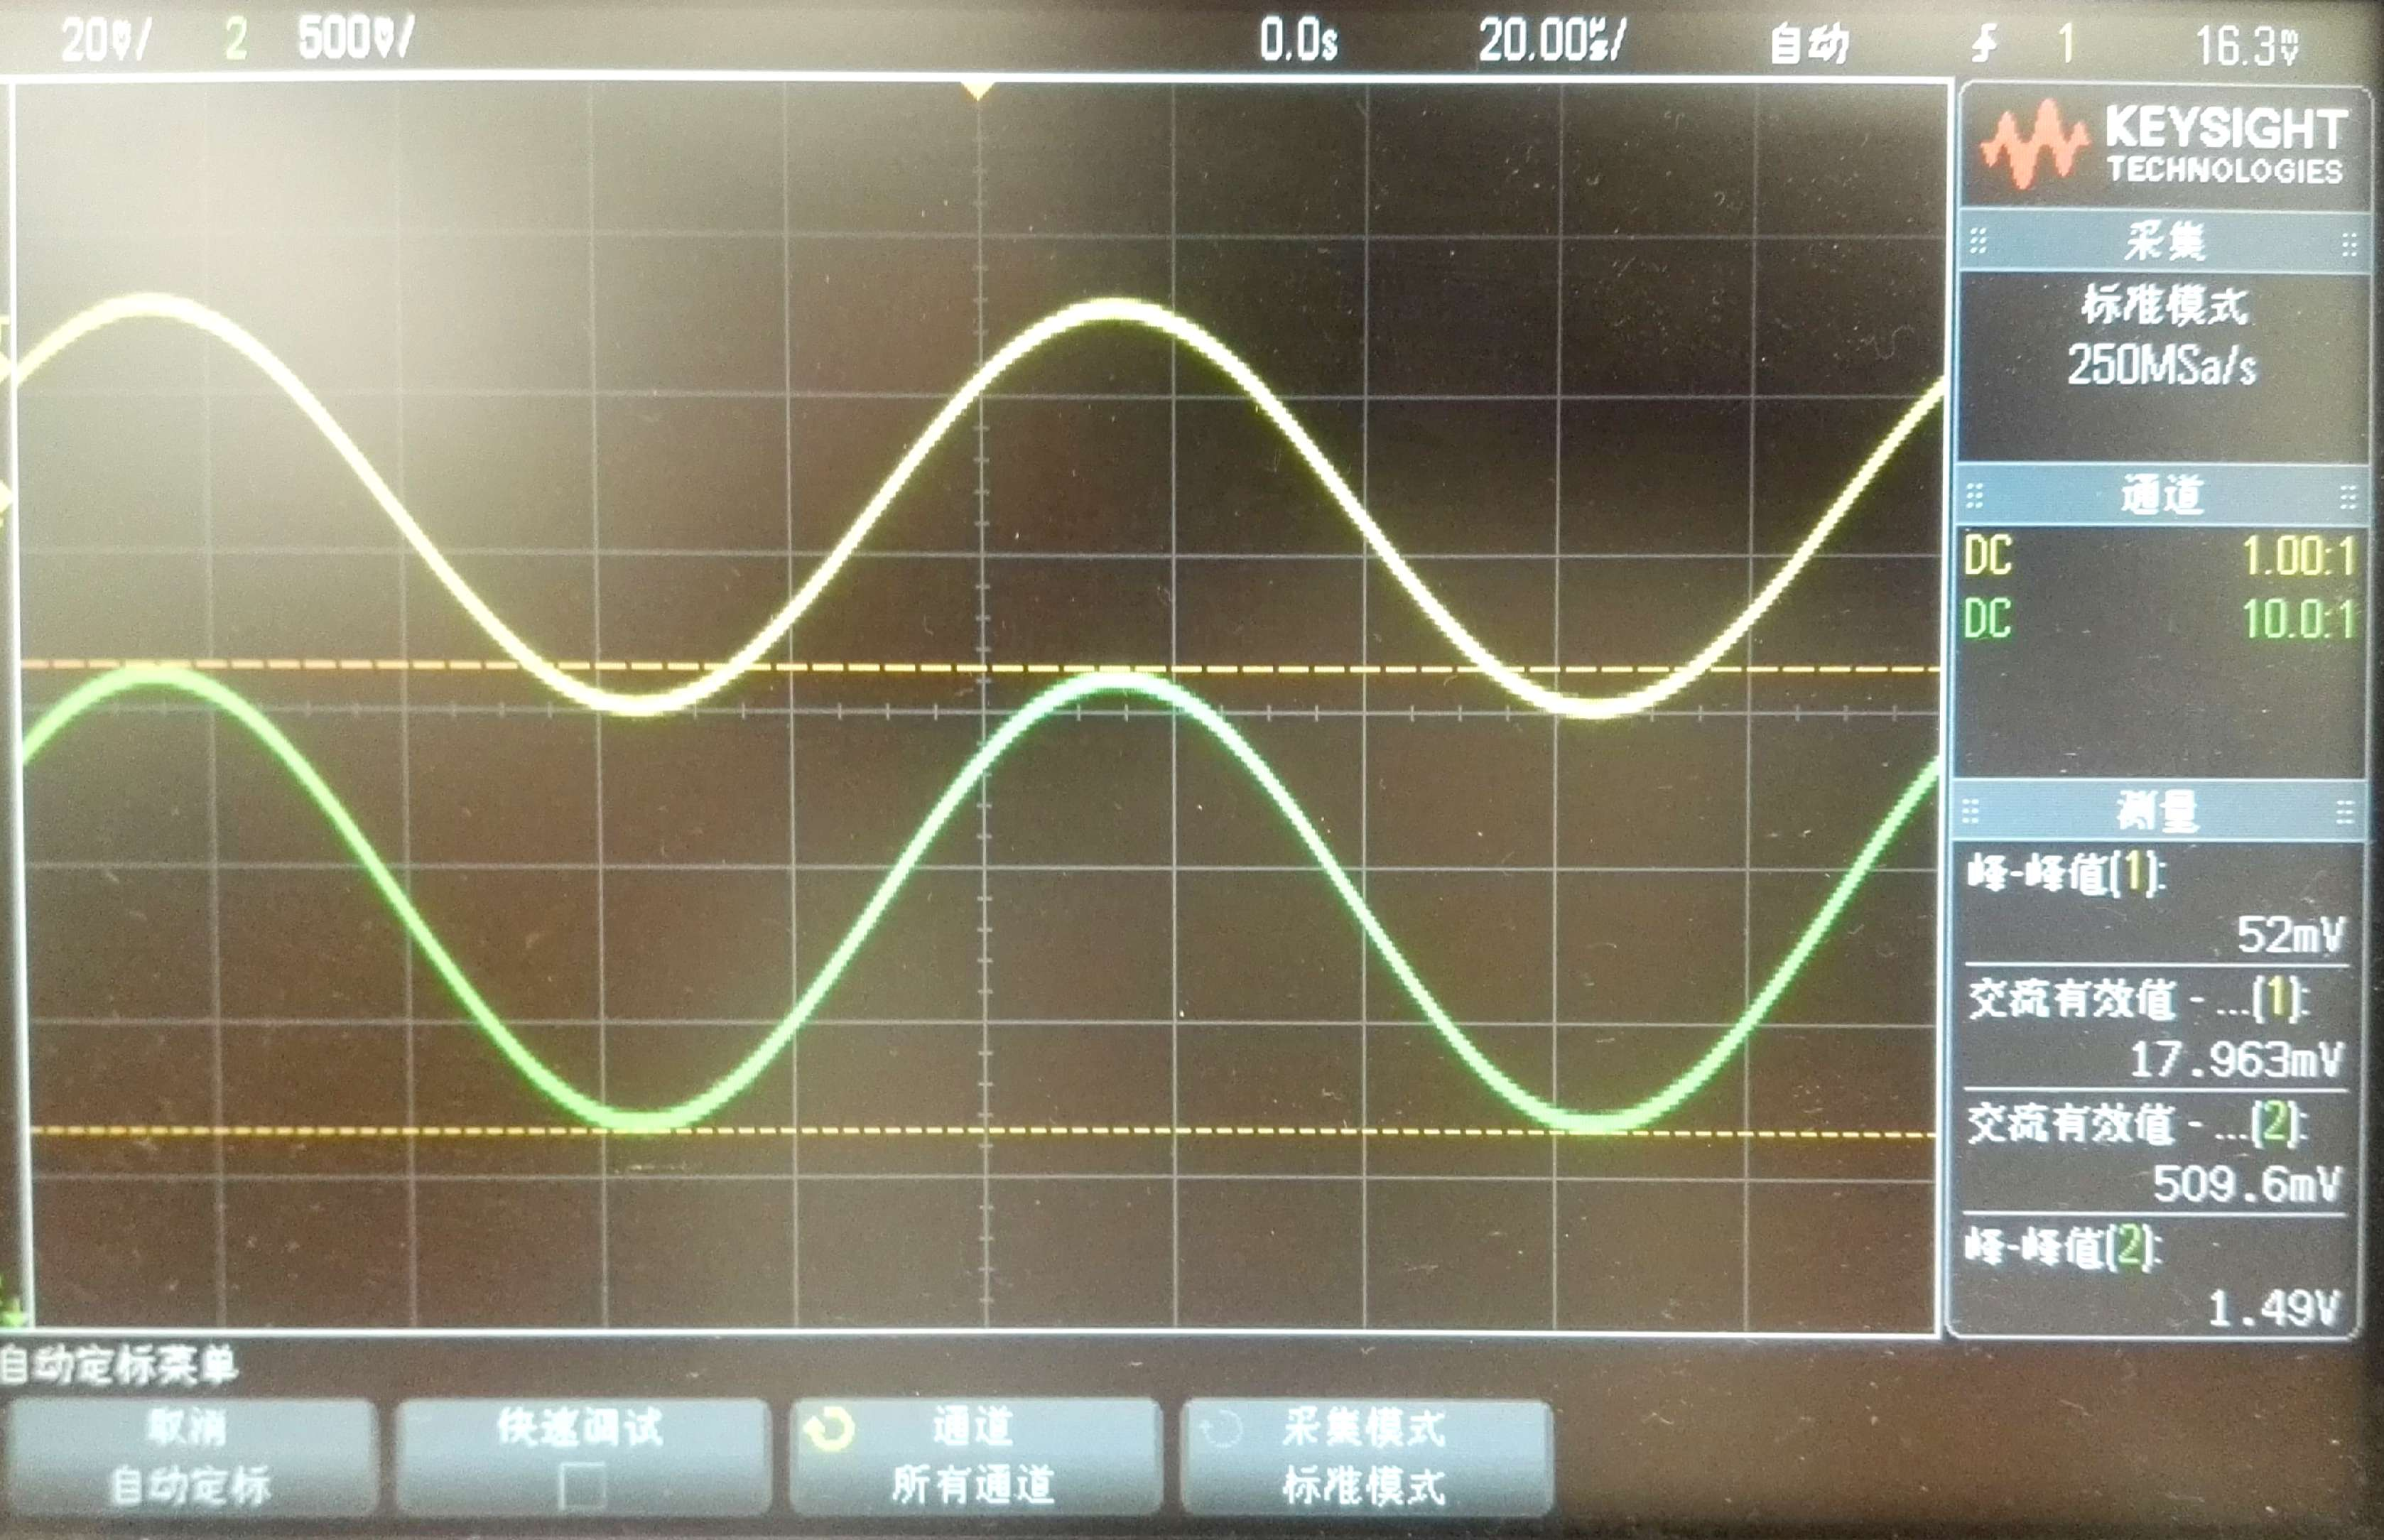
\includegraphics[width=\textwidth]{pic2.jpg}
\end{figure}
\begin{figure}[H]
\centering
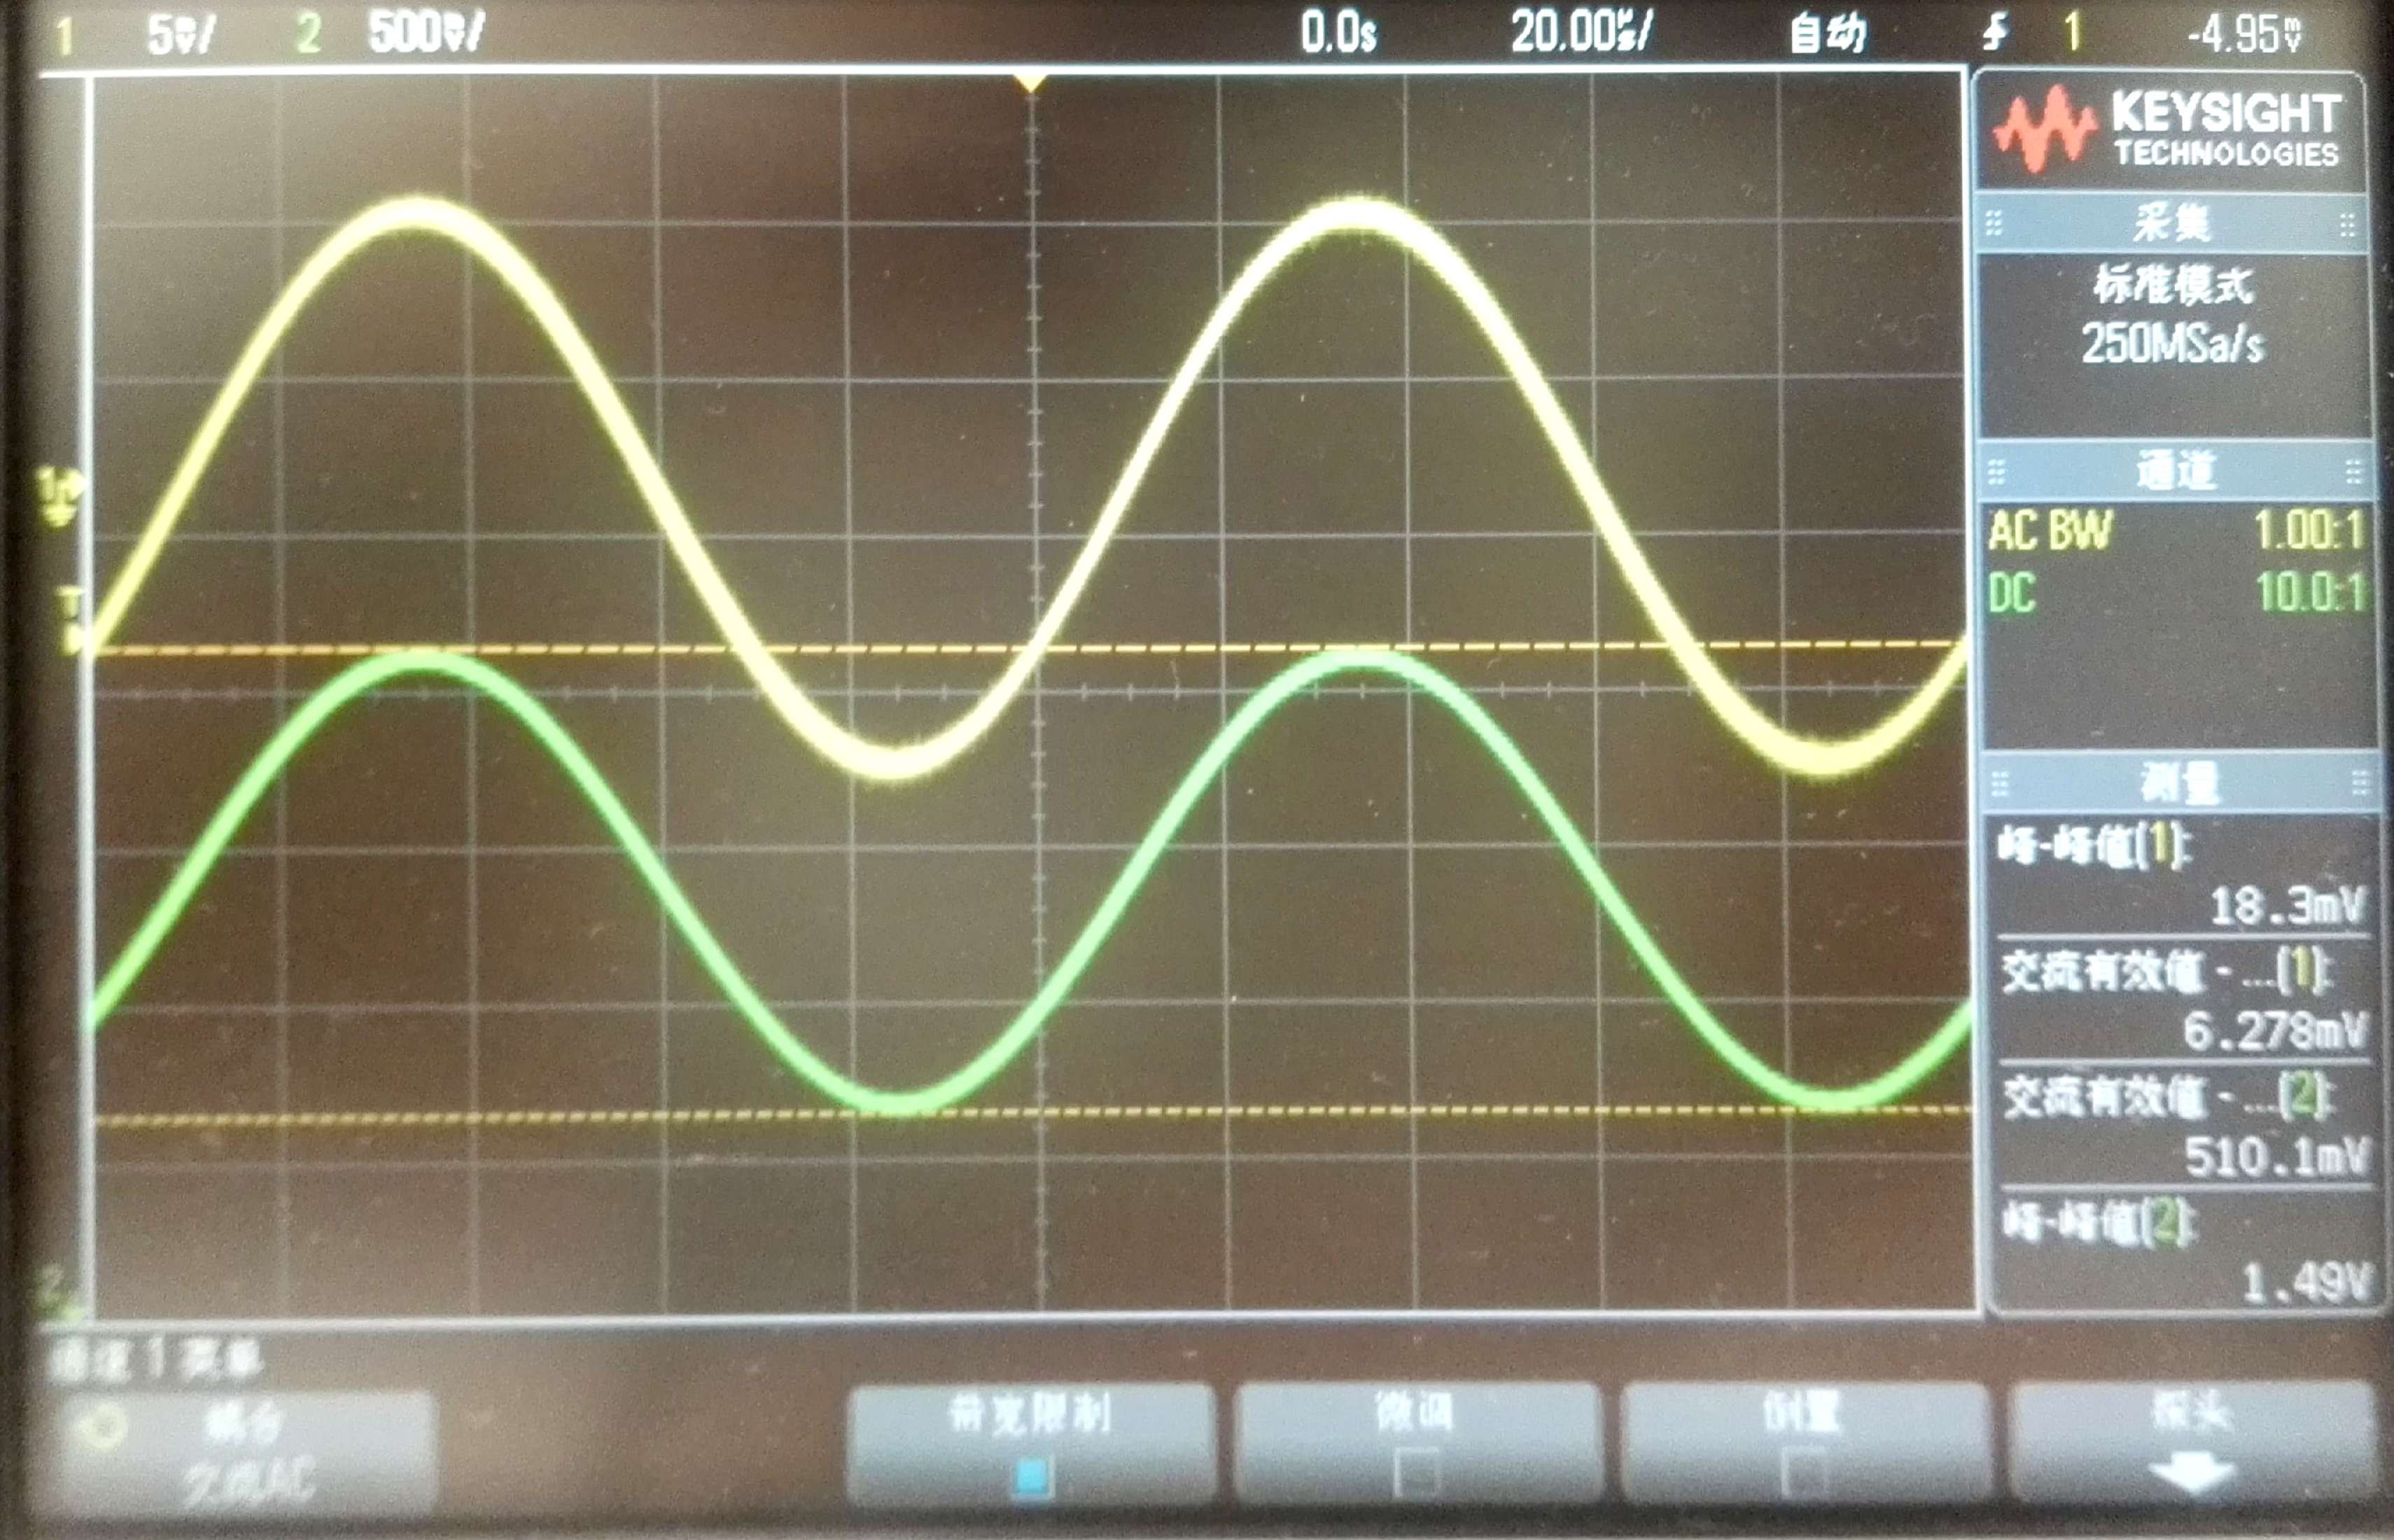
\includegraphics[width=\textwidth]{pic3.jpg}
\end{figure}
\paragraph{输出电阻} 方法与必做实验相同。开路时,$U_o = 609.3mV$;$R_L = 10k\Omega 时,U_{o}^{'}=459.4mV$,据此计算出$R_{of}=(\frac{609.3}{459.4}-1)\times 10k\approx 3.26k\Omega$。波形图如下。
\begin{figure}[H]
\centering
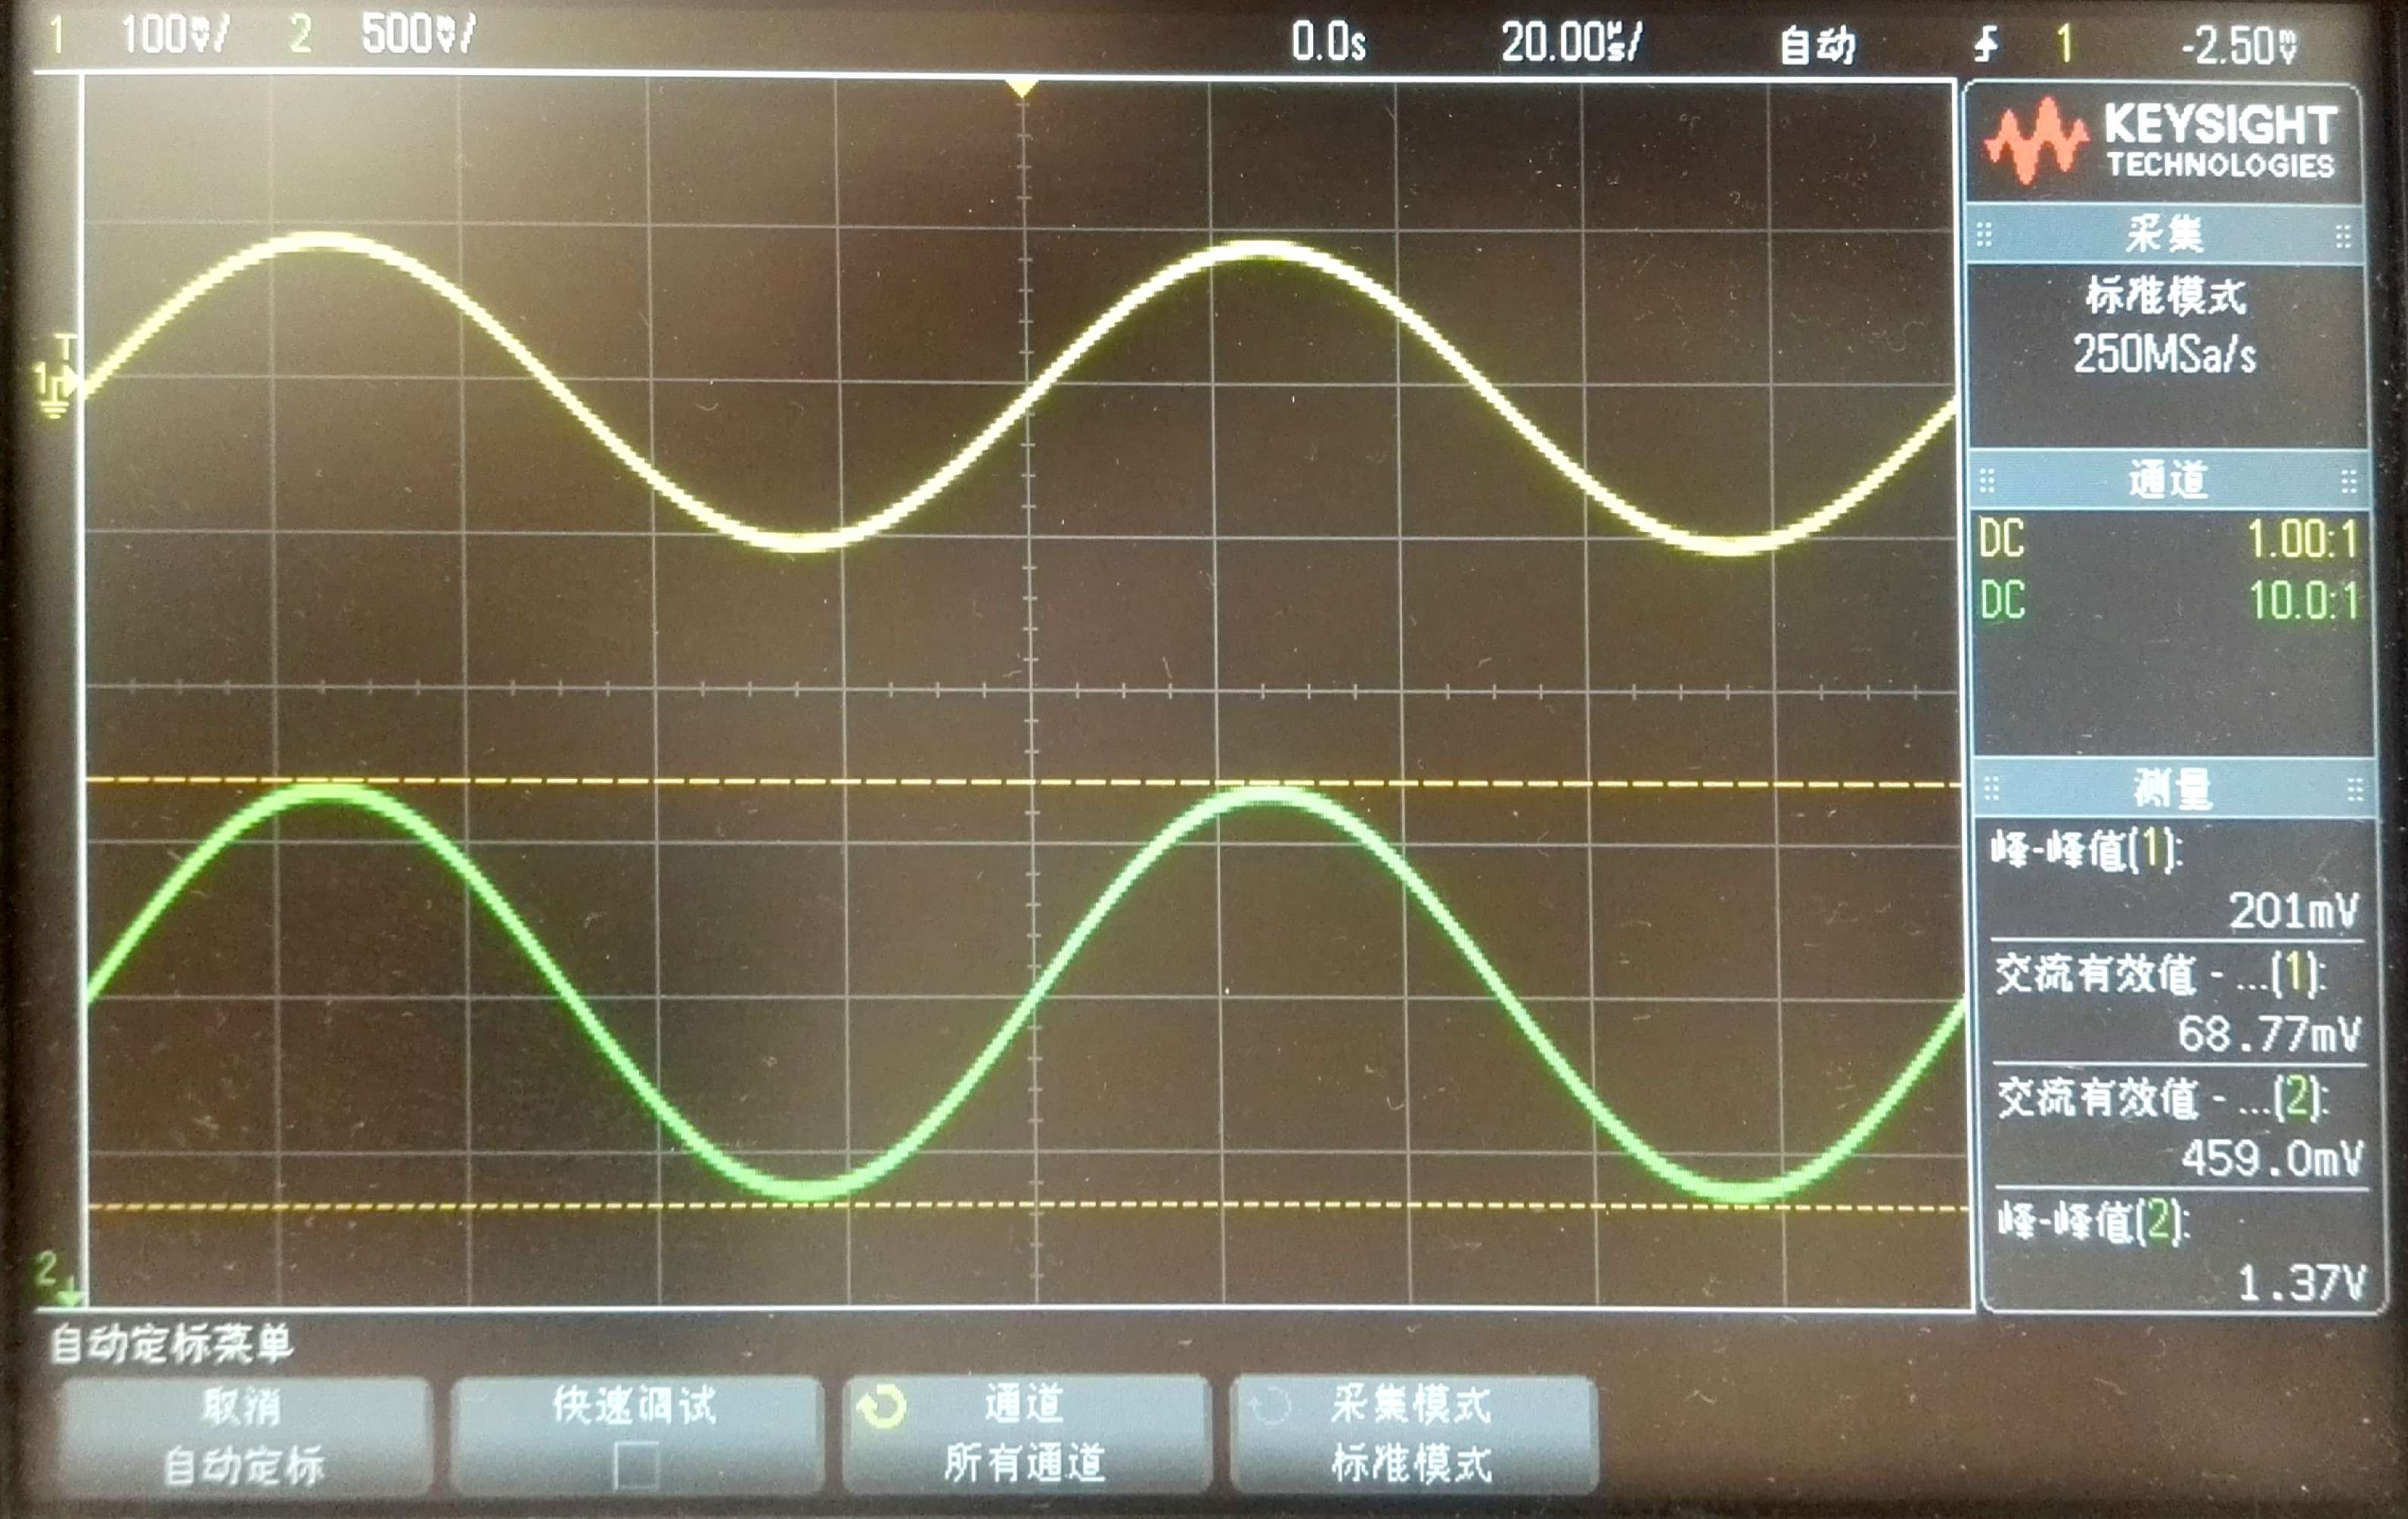
\includegraphics[width=\textwidth]{pic4.jpg}
\end{figure}
将理论、仿真、实验值整理为如下表格。可以看到,三者较为接近。
\begin{table} [H]
\centering
\begin{tabular}{|c|c|c|c|}
% hline draws a horizontal line
\hline 
&$\dot{A_{usf}}$ &$R_{if}(\Omega)$ &$ R_{of}(\Omega)$ \\ \hline 
理论值 &$12.1 $& $297.7 $ &$ 3.3k$\\ \hline
仿真值&$9.38 $& $ 307.95$ &$ 3.27k$\\ \hline 
实验值&$8.85 $& $372.4 $ &$ 3.26k$\\ \hline
\end{tabular} 
\end{table} 
\section{实验中遇到的问题及解决方法}
本次实验分两次完成。在第一次实验时间,顺利地恢复出两级放大电路并完成了必做实验。但选做实验花费大量时间调试第二级电路,导致在下课前没能做出。在开放时间,得益于秦俭老师的指点,对于问题得到了有效的解决。
\subsection{选做实验第一级电路波形下降的问题}
第一级电路的波形,在示波器上有时会随时间稳定地下降。这一问题十分令人困惑,最后不知什么原因波形重归于稳定。现在想来,如果将输入置为AC模式,这一问题可能会得到解决。
\subsection{选作实验第二级电路动态的问题}
第二级电路在第一次课和第二次课的调试中,均出现了第二级静态正确,动态却不能正常放大的问题。经秦俭老师提示,发现问题在于,在测试时输入没有经过电容耦合。所以,这相当于直接将三极管的基极接地,发射结没有正偏,当然不可能有正常的实验结果。最初以为电容对于交流通路等效于导线,可有可无,却忽略了它对直流通路的极端必要性。
\section{实验体会}
本次实验首先令我熟悉了负反馈放大电路的组态的概念,令我对负反馈、深度负反馈对电路性能的影响有了实验上的体会。另外,这次实验中令我印象尤为深刻的,是第二个问题的解决,这个问题反映出理论分析对于实验调试的重要指导意义。在实验波形的调试过程中,秦俭老师还为我介绍了Trigger稳定波形的原理,令我印象深刻。十分感谢助教和老师,特别是秦俭老师在这次实验中的帮助。
\end{spacing}
\end{document}
